\documentclass{article}
\usepackage[utf8]{inputenc}
\usepackage[english]{babel}


\setstretch{}
\usepackage[
backend=biber,
sorting=none
]{biblatex}
 
\addbibresource{references.bib}
 
 \usepackage
[
        a4paper,% other options: a3paper, a5paper, etc
        left=3cm,
        right=3cm,
        top=3cm,
        bottom=4cm,
        % use vmargin=2cm to make vertical margins equal to 2cm.
        % us  hmargin=3cm to make horizontal margins equal to 3cm.
        % use margin=3cm to make all margins  equal to 3cm.
]
{geometry}

\usepackage{setspace}
\usepackage[shortlabels]{enumerate}
 

\title{Teorispørsmål for Bølgeforplantning}
\author{TFE4130}
\date{Laget 13. Desember 2016}

%\usepackage{natbib}
\usepackage{graphicx}

\begin{document}

\maketitle

\begin{figure}[h!]
\centering
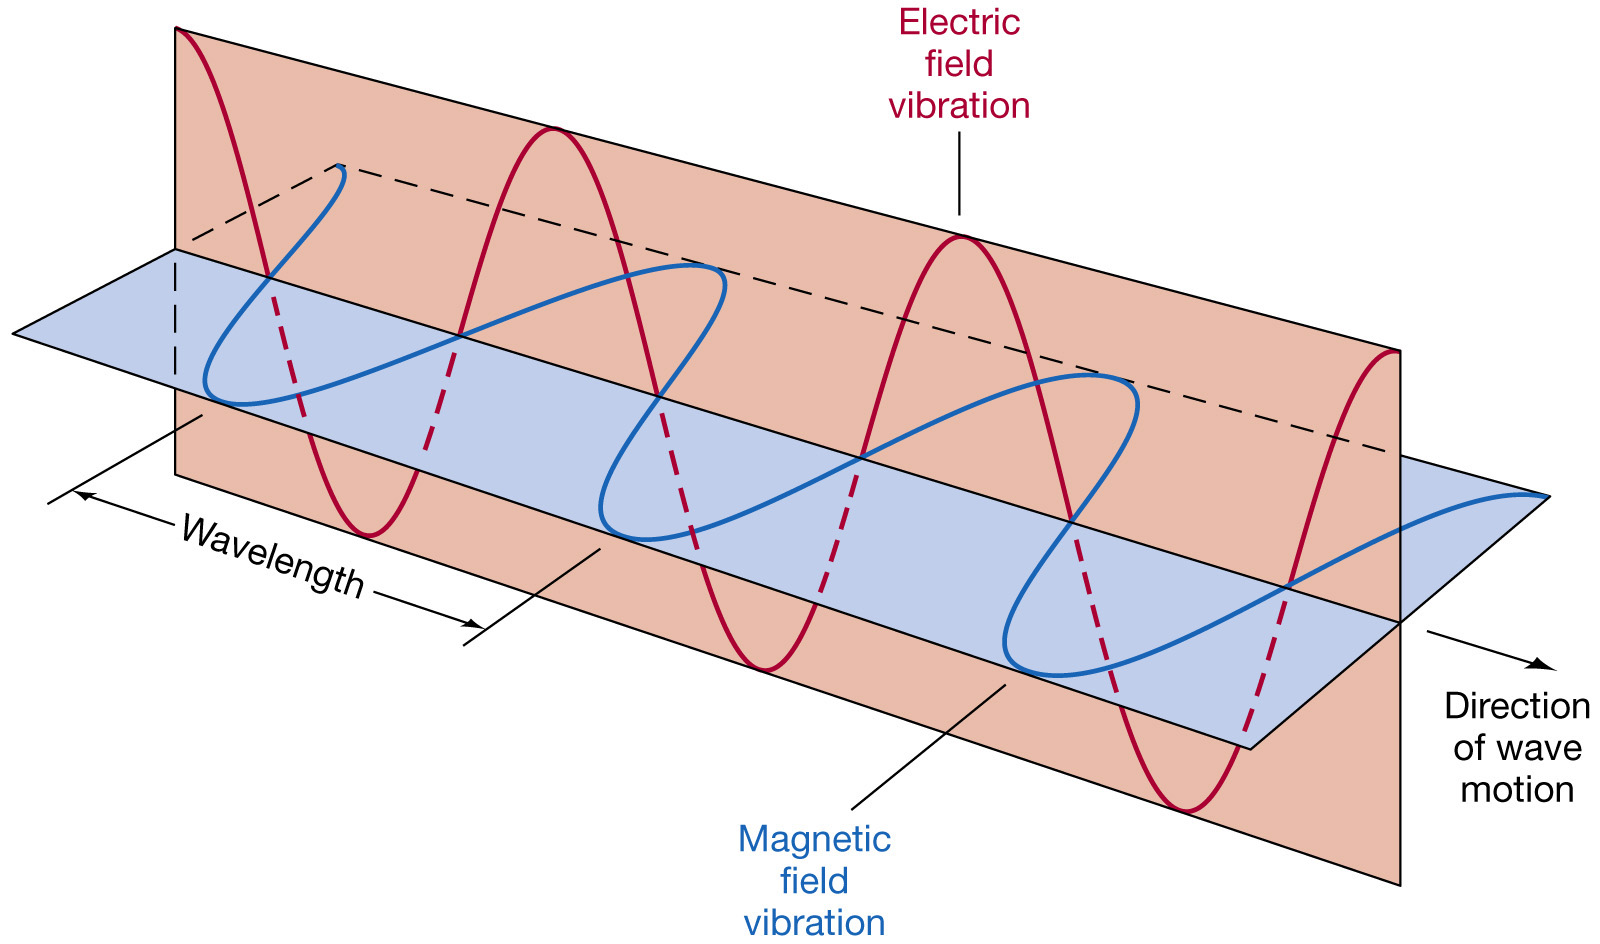
\includegraphics[scale=0.2]{wave_propagation.jpg}
\caption{TEM-bølge}
\label{fig:intro_pic}
\end{figure}

{\setstretch{2}
\section*{Introduksjon}
Dette dokumentet er laget som forberedelse til eksamen 21. Desember 2016 i faget Bølgeforplantning. 
Spørsmålene er hentet fra \textbf{Theory Problems for TFE4130}\cite{theory}. Svarene er laget av studenter ved studieprogrammet Elektronisk systemdesign og innovasjon\cite{elsys} ved NTNU. 
}

\section*{Bidra!}
For at dette dokumentet skal bli en god ressurs trenger vi at akkurat DU hjelper til! Ta for deg en oppgave du tror du kan løse og del svaret med dine medstudenter. Det er god juleånd det!

\newpage

\textbf{\section*{Problem 1}}

\begin{enumerate}[a)] 
\item Why are potential functions used in electromagnetics?\\
Svar: 
\item Express E and B in terms of potential functions V and A.\\
Svar: 
\item Derive the nonhomogeneous wave equation for the potential V. Clearly state the assumptions\\
Svar: 
you make.
\item Write down the expression for the retarded electric potential V and explain it.\\
Svar: 
\item Derive Helmholz’ equation and clearly state all the assumptions you make.\\
Svar: 
\end{enumerate}



\textbf{\section*{Problem 2}}

\begin{enumerate}[a)] 
\item Define, mathematically, a uniform plane wave and show that it is a solution to the Helmholz equation.\\
Svar: 
\item Show that $\textbf{E} \cdot \textbf{H} = 0$ for a harmonic plane wave.\\
Svar: 
\item State Poynting’s theorem. Provide an interpretation.\\
Svar: 
\item Two orthogonal linearly polarized waves are combined. State the conditions under which
the resultant will be i) another linearly polarized wave,ii) a circularly polarized wave and
iii) an elliptically polarized wave.\\
Svar: 
\item Define group and phase velocity. Derive the expression that relates ug with up.\\
Svar: 
\item What do the Fresnel equations express? Assume $\Gamma_\perp = −1/2$. What does this mean?\\
Svar: 

\end{enumerate}

\textbf{\section*{Problem 3}}
\begin{enumerate}[a)]

\item What are the three most common guiding structures that support TEM waves ?\\
Svar: 
\item  Derive the general transmission line equations (telegrapher’s equations) starting from
the circuit in Figure 1 and Kirchoff’s laws.\\
Svar: 

\item What is the phase relationship between the voltage and current waves on an infinitely
long transmission line?\\
Svar: 
\item What is the input impedance of an open-circuited lossless transmission line if the length
of the line is $\lambda/4?$\\
Svar: 


\end{enumerate}



\textbf{\section*{Problem 4}}
\begin{enumerate}[a)]

\item Why are the common types of transmission lines not useful for the long distance signal transmission at microwave frequencies in the TEM mode?\\
Svar:
\item What is meant by a cut-off frequency?\\
Svar:
\item What are the three basic types of propagating waves in a uniform waveguide?\\
Svar:
\item Derive the TE modes from Helmholz equation.\\
Svar:
\item Under what circumstances does a Bessel’s differential equation arise?\\
Svar:

\end{enumerate}

\textbf{\section*{Problem 5}}
\begin{enumerate}[a)]
\item Define a Hertzian dipole and derive its complete E&M field.\\
Svar:
\item Draw figures describing both an electric and a magnetic dipole. Discuss how their near and far field compares.\\
Svar:
\item Mathematically define directive gain and directivity for an antenna. You also need to define what we mean with a solid angle.\\
Svar:
\item Describe, and draw, the radiation pattern of a half-wave dipole antenna.\\
Svar:
\item Derive how the antenna pattern arrives from adding up many Hertzian dipole antennas.\\
Svar:

\end{enumerate}

\textbf{\section*{Problem 6}}
\begin{enumerate}[a)]
\item What assumptions go into deriving the wave equation for acoustic waves?\\
Svar:
\item Outline all the steps in deriving the wave equation for a gas.\\
Svar:
\item Derive the acoustic impedance for a backward traveling wave.\\
Svar:
\item Derive the transmission and reflection coefficients for an acoustic wave between two media with different acoustic impedances.\\
Svar:
\item Show how the far field of an acoustic/E\&M wave can be obtained as the Fourier transform of the antenna aperture.\\
Svar:

\end{enumerate}











%\bibliographystyle{plain}
%\bibliography{references}


\printbibliography

\end{document}
